\documentclass[letterpaper,12pt]{report}

\usepackage{graphicx}
\usepackage{hyperref}
\usepackage[top=1in, bottom=1in, left=1.25in, right=1in]{geometry}

\hypersetup{
    colorlinks, %set true if you want colored links
    linkcolor=black,  %choose some color if you want links to stand out
}

\begin{document}
	\title{SYSC4907 Project Proposal}
	\author{Real-Time Collaboration Messaging Application}
	\date{}
	\maketitle

	\begin{abstract}
		The students working on this project are Thao-Tran Le-Phuong, Honor
		Lopes, Riley MacKinnon, and Igor Veselinovic and their student numbers
		are 100997443, 101008909, 100996542, and 101011081, respectively. The
		supervisor for this project is Cheryl Schramm. This document will
		outline the objectives, tasks, and methods of the project, as well as
		describe the background context for the project itself. The proposal
		will also provide a projected timeline of the project and the
		facilities that will be required during the process. The relevance of
		the project to the degree of each student will be explained as well.
	\end{abstract}

	\tableofcontents

	\pagebreak

	\section*{Objectives}
	\markright{}
	\addcontentsline{toc}{section}{Objectives}
	The objective of this project is to develop a messaging platform where
	conversations start out as a blank document that allows for real-time
	collaboration between users. Real-time collaboration in the context of 
	a document meaning that when a user edits the document, other users will 
	be able to see that change instantly, and also make their own changes. 
	We aim to build upon current implementations of real-time collaboration 
	and extend those implementations to provide additional features.

	\section*{Background}
	\markright{}
	\addcontentsline{toc}{section}{Background}
	Real-time collaboration has been implemented as a feature in word
	processing software, such as Microsoft Word, Google Docs, and Pages. These
	applications provide a more professional and formal environment for
	document writing. Our project aims to provide a similar environment geared
	towards social interaction. VS Code currently implements an overview of the
	opened document to show the user which part of the document they are
	currently viewing. This feature is called a 'mini-map'. Our goal is to
	implement this feature to show where the other users are in the
	conversation as well as the user's relative position in the conversation.
	Current messaging applications follow a more rigid messaging format.
	Messages in a conversation are often presented in chronological order and 
	are immutable. Our application will strive to break from these conventions
	to provide a fully editable conversation where the user can type wherever
	they choose.

	\section*{Tasks}
	\markright{}
	\addcontentsline{toc}{section}{Tasks}
	This messaging application will allow users to create accounts to
	communicate with each other. The accounts can be created using an email
	account or with Google or Facebook authentication. When signed in, users
	can view and modify their conversations with other users.

	The base functionality of a conversation should mimic a real-time
	collaboration word processor. Any changes being made to the conversation
	will be reflected in real-time to all other users participating in the
	conversation. Text, images, and gifs will be accepted as valid conversation
	inputs. The application will support text styling options, such as bold,
	italics, underlines, etc. Conversation content can also be locked by users
	so that a specific group of content cannot be modified.

	In addition to the word processing capabilities, there will be features to
	supplement the messaging platform.  Users will be notified immediately when
	other users modify a conversation in the same vein as text message
	notifications. Upon re-entering a conversation, the user will be presented
	with the changes made since the last time they were active. Users can
	manually view the history of any excerpt to determine which user
	contributed each change to the excerpt. An overview of the conversation
	that displays the positions of other active users in the conversation, which 
	we have named the mini-map, will be placed in the corner of every 
	conversation.

	Search functionality will also be provided in the application. Users will
	be able to search through conversations for specific keywords and filter
	certain parameters.

	\section*{Methods}
	\markright{}
	\addcontentsline{toc}{section}{Methods}
	We will research and use many different software development methodologies,
	tools, and technologies in the process of building this system. Software
	development is an inherently volatile branch of engineering, so we will
	need a workflow that is flexible enough to accommodate for any sudden shifts
	in design. The Agile methodology would allow us to quickly write code, test
	it, and have it running in our "production" environment. In addition to our
	weekly meetings with our supervisor, we will have team meetings once a week
	to update each other on individual progress and share any discoveries.
	Also, we will consider pair programming, where two programmers write code
	together at one computer, as a potential technique for working
	collaboratively. When not working together in person, we will communicate
	over Slack.

	We plan to use an online Kanban board on GitHub to help organize our Agile
	workflow. The board will be a space for us to put tasks and organize them
	into columns according to each task's progress. GitHub will also be where
	we host our remote repositories for all of our source code and
	documentation. GitHub features like organizations, pull requests, and issue
	tracking will help keep our project organized.

	Prior to the design process, requirements must be clearly specified. UML
	diagrams will be a useful tool during this process as it will allow us
	to visualize the relationships within our system. Visualization would aid
	in preparing the system designs and clarifying requirements. Use cases for
	testing are also directly based off of the requirements so it is important
	that they are clear enough that the tests will validate the correct
	behaviour.

	Once code for a feature or bug fix is written by one team member (or two in
	the case of pair programming), it will need to go through code review by at
	least one other team member. Testing will also be an important step for
	validating new changes to any code base we have. Continuous
	Integration/Continuous Deployment (CI/CD) pipelines will help in automating
	this process. Before any pull request can get merged to our master branch
	in Git, it must be approved by at least one reviewer and a pipeline must be
	run that will run a suite of tests to validate that there are no breaking
	changes.

	Since we are developing a complex software system, we will need to research
	technologies for each component of the system. We need a scalable platform
	to run the server-side code, so cloud vendors like Amazon Web Services or
	Google Cloud could be useful options for us. The concurrency and memory
	management features of Go make it suitable for our server-side needs, along
	with a relational database management system using SQL. There are many
	framework options for the front-end of our web application, including
	React, Angular, and Vue. WebAssembly is another front-end technology that
	we are interested in incorporating into our web application.

	\section*{Timetable}
	\markright{}
	\addcontentsline{toc}{section}{Timetable}
	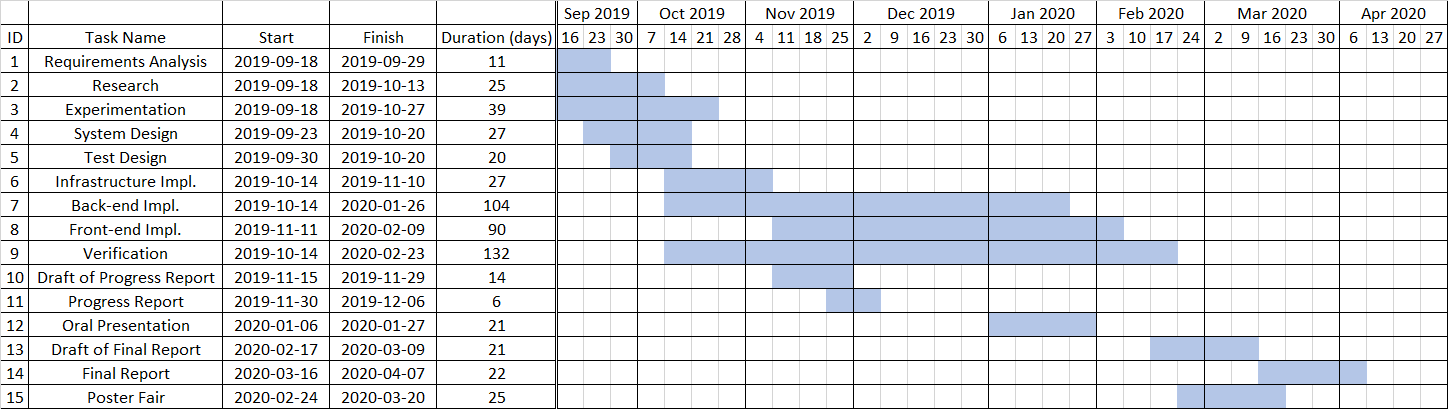
\includegraphics[width=\linewidth]{timetable.png}

	\section*{Facilities}
	\markright{}
	\addcontentsline{toc}{section}{Facilities}
	We will be running server-side code on a cloud hosting service. Hosts such
	as Amazon Web Services offer free trials for the first year, which would
	cover the length of this project. If these services are unavailable for
	free, we would expect our hosting costs to be less than \$100. This project
	would benefit from having a workplace available for us to work in. It would
	help to have an on-campus space to develop in.

	\section*{Degree Relevance}
	\markright{}
	\addcontentsline{toc}{section}{Degree Relevance}

	\subsection*{Thao-Tran Le-Phuong}
	\markright{}
	\addcontentsline{toc}{subsection}{Thao-Tran Le-Phuong}
	This project is an application of many topics learned and developed in the
	Computer Systems Engineering degree. This project will involve the entire
	software development process, including requirements, planning,
	development, testing, verification, and maintenance. This degree requires
	multiple programming courses to be taken and the knowledge learned in these
	courses will be applied when implementing this software. This project is
	real-time and responds to unpredictable inputs from multiple users as
	discussed in courses taken. This project will involve the use of cloud
	hosting and processing services, which is a current industry topic.

	\subsection*{Honor Lopes}
	\markright{}
	\addcontentsline{toc}{subsection}{Honor Lopes}
	This project is an application of many topics learned and developed in the
	Computer Systems Engineering degree. This project will involve the entire
	software development process, including requirements, planning,
	development, testing, verification, and maintenance. This degree requires
	multiple programming courses to be taken and the knowledge learned in these
	courses will be applied when implementing this software. This project is
	real-time and responds to unpredictable inputs from multiple users as
	discussed in courses taken. This project will involve the use of cloud
	hosting and processing services, which is a current industry topic.

	\subsection*{Riley MacKinnon}
	\markright{}
	\addcontentsline{toc}{subsection}{Riley MacKinnon}
	This project is an application of many topics learned and developed in the
	Software Engineering degree. This project will involve the entire software development
	process, including requirements, planning, development, testing,
	verification, and maintenance. This degree requires multiple programming
	courses to be taken and the knowledge learned in these courses will be
	applied when implementing this software. This project is real-time and
	responds to unpredictable inputs from multiple users as discussed in
	courses taken. This project will involve the use of cloud hosting and
	processing services, which is a current industry topic. The database for
	this software will be written in SQL with the design and methods learned
	from database management courses.

	\subsection*{Igor Veselinovic}
	\markright{}
	\addcontentsline{toc}{subsection}{Igor Veselinovic}
	This project is an application of many topics learned and developed in the
	Computer Systems Engineering degree. This project will involve the entire
	software development process, including requirements, planning,
	development, testing, verification, and maintenance. This degree requires
	multiple programming courses to be taken and the knowledge learned in these
	courses will be applied when implementing this software. This project is
	real-time and responds to unpredictable inputs from multiple users as
	discussed in courses taken. This project will involve the use of cloud
	hosting and processing services, which is a current industry topic.
\end{document}
